\documentclass[11pt,letterpaper]{article}
\usepackage[margin=0.85in]{geometry}
\usepackage[T1]{fontenc}
\usepackage[utf8]{inputenc}
\usepackage{lmodern,microtype}
\usepackage{amsmath,amssymb}
\usepackage{booktabs,tabularx,array}
\usepackage{graphicx,float}
\usepackage{tikz}
\usetikzlibrary{positioning,arrows.meta}
\usepackage{xcolor,hyperref,caption,fancyhdr,enumitem,listings}
\definecolor{navy}{HTML}{233B55}
\definecolor{teal}{HTML}{147D81}
\definecolor{rust}{HTML}{B85B27}
\definecolor{soft}{HTML}{F2F5F7}
\hypersetup{colorlinks=true,linkcolor=navy,urlcolor=teal,citecolor=navy,pdftitle={Deep Learning Midterm Project Report},pdfauthor={Vinay Kumar Uppalapati}}
\setlength{\parindent}{0pt}
\setlength{\parskip}{5pt}
\setlength{\headheight}{14pt}
\renewcommand{\arraystretch}{1.16}
\setlist[enumerate]{leftmargin=1.5em,itemsep=1pt,topsep=2pt}
\pagestyle{fancy}\fancyhf{}
\fancyhead[L]{\footnotesize Deep Learning Midterm Project}
\fancyhead[R]{\footnotesize Vinay Kumar Uppalapati}
\fancyfoot[C]{\thepage}
\renewcommand{\headrulewidth}{0.3pt}
\captionsetup{font=small,labelfont=bf}
\lstset{basicstyle=\ttfamily\footnotesize,breaklines=true,frame=single,rulecolor=\color{gray!35},backgroundcolor=\color{soft},showstringspaces=false,columns=fullflexible}
\begin{document}
\begin{center}
{\Large\bfseries\color{navy} Comparative Analysis of Transformer Models for Health Claim Verification:\par}
\vspace{2pt}
{\large\bfseries\color{navy} Accuracy, Data Efficiency, and Error Patterns\par}
\vspace{8pt}
{Vinay Kumar Uppalapati}\quad |\quad Deep Learning Midterm Project\\
{\small November 2026}
\end{center}
\hrule\vspace{6pt}

\noindent\textbf{Project summary.} For this midterm, I fine-tuned SciBERT and DistilBERT on HealthVer to classify whether scientific evidence supports, refutes, or is neutral toward a health claim. I compared them with a TF-IDF + Logistic Regression baseline and tested 25\%, 50\%, and 100\% of the training data. SciBERT performed best, reaching \textbf{76.14\% accuracy} and \textbf{0.7475 Macro-F1} on the test set. The experiments also showed how training loss can keep decreasing even when development performance stops improving.

\section{Introduction: What I Wanted to Learn}
My project examines whether a piece of evidence \textbf{supports}, \textbf{refutes}, or is \textbf{neutral} toward a health-related claim. The model must judge the relationship between the two texts, not establish whether the claim is medically true in every context.

I chose HealthVer \cite{sarrouti} because it provides labeled claim-evidence pairs for this task. SciBERT was my main model because it uses BERT's encoder architecture and was pretrained on scientific text \cite{beltagy}. I also fine-tuned the smaller DistilBERT model and trained a traditional machine-learning baseline. My aim was to study the architecture in a working system, compare its performance, and interpret the results. Since the HealthVer researchers had already evaluated SciBERT, I treated this as a controlled class experiment rather than a new research method.

\section{Dataset Preparation}
\subsection{What the dataset looks like}
HealthVer contains \textbf{14,330} claim-evidence pairs, mainly related to COVID-19 questions \cite{sarrouti}. I used the \texttt{claim} and \texttt{evidence} fields as inputs and \texttt{label} as the target. Labels were mapped to SUPPORT = 0, REFUTE = 1, and NEUTRAL = 2. NEUTRAL means that the supplied evidence does not establish support or refutation, it does not mean the claim is false.

I loaded the official train, development, and test files. The notebook checked for missing or empty text, removed surrounding spaces, and standardized labels. These checks removed no rows. I kept the original splits separate.

\begin{table}[H]
\centering\small
\caption{Class distribution in my prepared dataset.}
\begin{tabular}{@{}lrrrr@{}}\toprule
\textbf{Split} & \textbf{SUPPORT} & \textbf{REFUTE} & \textbf{NEUTRAL} & \textbf{Total}\\\midrule
Training & 3,782 & 2,411 & 4,397 & 10,590\\
Development & 533 & 391 & 993 & 1,917\\
Test & 671 & 425 & 727 & 1,823\\\midrule
Total & 4,986 & 3,227 & 6,117 & 14,330\\\bottomrule
\end{tabular}
\end{table}

I used training data to update model weights, development data to select checkpoints, and the test set for final reporting. The REFUTE class has fewer examples than the other two classes, so I included Macro-F1 rather than relying on accuracy alone.

\subsection{How the model receives text}
SciBERT's tokenizer converts the claim and evidence into subword tokens and numerical IDs. The combined input has the form

\[
[\mathrm{CLS}]\quad\mathrm{claim}\quad[\mathrm{SEP}]\quad\mathrm{evidence}\quad[\mathrm{SEP}].
\]
The \texttt{[CLS]} token is used for classification, and \texttt{[SEP]} marks the boundaries between texts. An attention mask distinguishes real tokens from padding. I limited the combined input to \textbf{256 tokens} and used dynamic padding within each batch. Longer pairs were truncated, potentially removing relevant evidence.

When inspecting the input, I noticed that a term such as \emph{hydroxychloroquine} was split into several subword tokens. This matters because tokenization determines the units the model uses to represent scientific terms. For the TF-IDF baseline, I joined the claim and evidence and used unigram and bigram features instead of contextual embeddings.

\subsection{Why I created three training sizes}
To examine data efficiency, I prepared class-stratified training subsets of \textbf{25\%, 50\%, and 100\%} containing 2,647, 5,295, and 10,590 examples. The smaller subsets were nested within the larger ones. Development (1,917 examples) and test (1,823 examples) sets stayed unchanged, allowing a consistent comparison as training data increased.

\section{Understanding the Transformer Architecture}
\subsection{SciBERT from input to prediction}
SciBERT follows the BERT-base encoder design, with \textbf{12 encoder layers}, \textbf{12 attention heads} per layer, a \textbf{768-dimensional hidden representation}, and about \textbf{109.9 million parameters} including the classification head. Transformers introduced attention-based sequence modeling, and BERT developed a bidirectional encoder \cite{vaswani,devlin}, SciBERT adapted BERT to scientific text \cite{beltagy}.

Working with SciBERT reinforced the encoder-only and decoder-only distinction covered in class. This task needs one classification decision based on both texts, rather than generating a sequence, so a bidirectional encoder is a suitable choice. Token embeddings pass through the encoder layers, and the final classification head produces three scores, as shown below.

\begin{figure}[H]
\centering
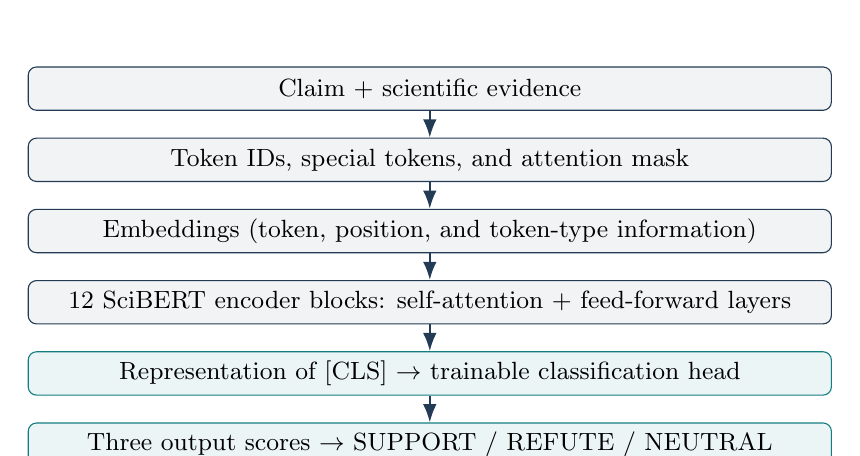
\begin{tikzpicture}[>=Latex,node distance=0.34cm,every node/.style={font=\small},
b/.style={draw=navy,fill=navy!6,rounded corners=3pt,minimum width=10.2cm,minimum height=0.55cm,align=center},
c/.style={draw=teal,fill=teal!8,rounded corners=3pt,minimum width=10.2cm,minimum height=0.55cm,align=center}]
\node[b] (a) {Claim + scientific evidence};
\node[b,below=of a] (bb) {Token IDs, special tokens, and attention mask};
\node[b,below=of bb] (cc) {Embeddings (token, position, and token-type information)};
\node[b,below=of cc] (dd) {12 SciBERT encoder blocks: self-attention + feed-forward layers};
\node[c,below=of dd] (ee) {Representation of [CLS] $\rightarrow$ trainable classification head};
\node[c,below=of ee] (ff) {Three output scores $\rightarrow$ SUPPORT / REFUTE / NEUTRAL};
\foreach \x/\y in {a/bb,bb/cc,cc/dd,dd/ee,ee/ff}{\draw[->,thick,navy] (\x)--(\y);}
\end{tikzpicture}
\caption{Simplified view of the actual SciBERT classification workflow.}
\end{figure}


\subsection{Self-Attention and Its Role in Claim Verification}

Self-attention lets each token build a representation using information from other tokens in the sequence. SciBERT processes the claim and evidence together, so it can consider the relationship between them. For example, \emph{reduces} and \emph{did not reduce} describe different outcomes despite sharing most words. Attention can represent this difference, although it does not guarantee correct classification of every negation.

The scaled dot-product attention mechanism is expressed as:

\begin{equation}
\operatorname{Attention}(Q,K,V)
=
\operatorname{softmax}
\left(
\frac{QK^\top}{\sqrt{d_k}}
\right)V.
\end{equation}

Here $Q$, $K$, and $V$ are query, key, and value matrices produced by learned projections. The product $QK^\top$ measures token relationships, scaling by $\sqrt{d_k}$ controls score size, and softmax produces weights for combining the value vectors.

SciBERT uses multi-head attention, followed by a feed-forward network, residual connections, and layer normalization in each encoder block. These are trainable transformations rather than fixed rules. Fine-tuning updates their weights through backpropagation, connecting the attention mechanism from class to my actual classification task. I did not inspect individual attention maps, so I cannot claim which tokens specific heads focused on.

\subsection{Embeddings and the classification layer}
Token IDs are mapped to learned embeddings, while position and token-type embeddings indicate word order and distinguish the two input segments. The contextual \texttt{[CLS]} representation passes to a classification head, which produces three \textbf{logits}. Softmax can turn them into class scores, but these are not necessarily calibrated probabilities of medical truth.

DistilBERT uses \textbf{6 encoder layers}, 12 attention heads, a 768-dimensional hidden size, and about \textbf{67 million parameters}. Since the two models differ in size and pretraining data, their performance difference cannot be attributed to scientific pretraining alone.

\section{Loss Function and Model Training}
\subsection{Cross-entropy loss, explained simply}
With three mutually exclusive labels, I used \textbf{cross-entropy loss}. It penalizes the model when it assigns low probability to the correct class. For one example,

\begin{equation}
L=-\sum_{k=1}^{3}\mathbf{1}(y=k)\log(p_k)=-\log(p_y),
\end{equation}
where $y$ is the correct label and $p_y$ is the softmax score for that label. For a batch of $N$ examples, the model averages the individual losses:
\begin{equation}
L_{\mathrm{batch}}=\frac{1}{N}\sum_{i=1}^{N}-\log\bigl(p_{i,y_i}\bigr).
\end{equation}
For example, if SUPPORT is correct, assigning it probability 0.90 gives a loss of $-\log(0.90)\approx0.105$, while assigning 0.10 gives $-\log(0.10)\approx2.303$. These are illustrative values, not predictions from my dataset. This reinforced why cross-entropy fits classification better than a regression loss such as MSE in this task.

In my notebook, the Hugging Face classifier returned the loss as \texttt{outputs.loss} when I supplied labels. It handles log-softmax internally, so I passed the logits directly without applying softmax first.

\subsection{Connection to code and backpropagation}
The following lines are selected from my transformer training code. They are shown without the surrounding data-loader setup:
\begin{lstlisting}[caption={Selected PyTorch/Hugging Face code used for fine-tuning.}]
model = AutoModelForSequenceClassification.from_pretrained(
    checkpoint, num_labels=3, id2label=ID_TO_LABEL,
    label2id=LABEL_TO_ID).to(device)
optimizer = torch.optim.AdamW(model.parameters(),
    lr=LEARNING_RATE, weight_decay=WEIGHT_DECAY)
outputs = model(**batch)
loss = outputs.loss
\end{lstlisting}
The code loads pretrained weights and a three-class output head. In the forward pass, the model computes predictions and cross-entropy loss. Backpropagation then calculates parameter gradients, and AdamW uses them to update both the encoder and classification head. This matches the distinction made in class between calculating gradients and using an optimizer to change weights.

\subsection{Training settings I actually used}
Both transformers were fine-tuned for up to three epochs on a Tesla T4 GPU in Google Colab. My saved settings were as follows:
\begin{table}[H]
\centering\small
\caption{Configuration used for the SciBERT and DistilBERT runs.}
\begin{tabular}{@{}ll@{}}\toprule
\textbf{Setting} & \textbf{Value}\\\midrule
Maximum sequence length & 256 tokens\\
Training batch size & 8\\
Gradient accumulation steps & 2 (effective batch about 16)\\
Evaluation batch size & 16\\
Epochs & 3\\
Optimizer & AdamW\\
Initial learning rate & $2\times10^{-5}$\\
Weight decay & 0.01\\
Learning-rate schedule & 10\% warmup, then linear decrease\\
Gradient clipping & Maximum norm of 1.0\\
Mixed precision & Enabled on GPU\\
Random seed & 42\\
Best checkpoint & Highest development Macro-F1\\\bottomrule
\end{tabular}
\end{table}

Gradient accumulation let me process two batches of 8 before an optimizer update, giving an effective batch size of about 16. I also used learning-rate warmup followed by linear decay. This training setup reinforced the roles of the optimizer and scheduler discussed in class.

The training curves later raised a question about overfitting: training loss kept decreasing while development loss rose. This connects to the class discussion of weight decay, dropout, and checkpoint selection. I did not implement patience-based early stopping, I trained for three epochs and kept the checkpoint with the best development Macro-F1.

For the traditional baseline, I used TF-IDF unigrams and bigrams (up to 50,000 features) followed by scikit-learn Logistic Regression.

\section{My Nine Experiments and Results}
\subsection{Why I used both accuracy and Macro-F1}
I evaluated three methods at three training sizes, giving \textbf{nine experiments}. All used the same 1,823-example test set. Accuracy measures the fraction correct. Precision and recall describe performance for individual labels, and F1 combines the two:

\[
F1=\frac{2\,\mathrm{Precision}\,\mathrm{Recall}}{\mathrm{Precision}+\mathrm{Recall}},
\qquad \mathrm{Macro\text{-}F1}=\frac{F1_S+F1_R+F1_N}{3}.
\]
Macro-F1 averages the three class F1 scores equally, which is useful because their frequencies differ.

\begin{table}[H]
\centering\small
\caption{Actual test results from the saved experiment CSV files.}
\begin{tabular}{@{}llrr@{}}\toprule
\textbf{Model} & \textbf{Data fraction} & \textbf{Accuracy (\%)} & \textbf{Macro-F1}\\\midrule
SciBERT & 25\% & 66.54 & 0.6437\\
SciBERT & 50\% & 71.53 & 0.6976\\
\textbf{SciBERT} & \textbf{100\%} & \textbf{76.14} & \textbf{0.7475}\\
DistilBERT & 25\% & 56.12 & 0.5358\\
DistilBERT & 50\% & 60.34 & 0.5877\\
DistilBERT & 100\% & 67.69 & 0.6664\\
TF-IDF + LR & 25\% & 58.69 & 0.5448\\
TF-IDF + LR & 50\% & 63.30 & 0.5974\\
TF-IDF + LR & 100\% & 66.43 & 0.6322\\\bottomrule
\end{tabular}
\end{table}


\begin{figure}[H]
    \centering
    \includegraphics[width=0.88\linewidth]{data_efficiency_macro_f1.png}
    \caption{Comparison of test Macro-F1 scores for SciBERT, DistilBERT, and TF-IDF with Logistic Regression using 25\%, 50\%, and 100\% of the training data.}
    \label{fig:data_efficiency}
\end{figure}


All three models improved as training data increased. SciBERT achieved the highest Macro-F1 at every fraction. At 100\%, it exceeded DistilBERT by 0.0811 and Logistic Regression by 0.1153. This shows its advantage in these experiments, although it does not establish that it would perform best on every dataset.

\subsection{Why the loss curves were interesting}
For SciBERT trained with 100\% of the data, training loss decreased across three epochs, but development loss increased. The lowest development loss was at epoch 1 (0.6811), while the highest development Macro-F1 was at epoch 2 (0.7222). Because checkpoint selection used Macro-F1, I kept epoch 2. The two metrics favored different epochs because cross-entropy uses confidence in the correct label, while F1 depends on final predicted labels.

\begin{table}[H]
\centering\small
\caption{Actual SciBERT training history at 100\% training data.}
\begin{tabular}{@{}rrrr@{}}\toprule
\textbf{Epoch} & \textbf{Training loss} & \textbf{Development loss} & \textbf{Development Macro-F1}\\\midrule
1 & 0.7181 & \textbf{0.6811} & 0.6778\\
\textbf{2} & 0.2986 & 0.7698 & \textbf{0.7222}\\
3 & 0.1536 & 0.9406 & 0.7022\\\bottomrule
\end{tabular}
\end{table}

\begin{figure}[H]
    \centering
    \includegraphics[width=0.84\linewidth]{scibert_100pct_loss_curve.png}
    \caption{Training and development loss from the 100\%-data SciBERT run.}
    \label{fig:scibert_loss_curve}
\end{figure}

This reinforced why fitting the training set more closely does not automatically mean better generalization. Rising development loss may indicate overfitting or increasingly confident mistakes.

\subsection{What the confusion matrix showed}
The best SciBERT model correctly classified \textbf{1,388 of 1,823} test examples. I used its confusion matrix to see which labels caused problems.

\begin{table}[H]
\centering\small
\caption{SciBERT confusion matrix at 100\% training data. Rows are true labels, columns are predicted labels.}
\begin{tabular}{@{}lrrr@{}}\toprule
 & \multicolumn{3}{c}{\textbf{Predicted}}\\\cmidrule(l){2-4}
\textbf{Actual} & \textbf{SUPPORT} & \textbf{REFUTE} & \textbf{NEUTRAL}\\\midrule
SUPPORT & \textbf{520} & 90 & 61\\
REFUTE & 92 & \textbf{278} & 55\\
NEUTRAL & 88 & 49 & \textbf{590}\\\bottomrule
\end{tabular}
\end{table}

REFUTE had the lowest class-wise F1 (\textbf{0.6603}), compared with 0.7586 for SUPPORT and 0.8234 for NEUTRAL. The model confused REFUTE with SUPPORT 92 times and SUPPORT with REFUTE 90 times. REFUTE is less common in training, but these results alone do not establish why it was more difficult.

\section{My Interpretations, Questions, and Discoveries}

\textbf{Tokenization and contextual representation.} I was already familiar with subword tokenization and attention, but implementing SciBERT showed me how practical choices affect this particular task. Combining claim and evidence in one sequence enables contextual interaction, while the 256-token limit may remove information from longer evidence passages. The TF-IDF comparison also made the difference between contextual representations and word-pattern features clearer.

\textbf{What I noticed about data size.} More labeled data helped all three models, which was expected. I found it more interesting that SciBERT remained ahead even with only 25\% of the data. This is consistent with pretrained scientific representations being useful, but the experiment cannot separate the effects of pretraining domain and model size.

\textbf{Training and generalization.} The mismatch between decreasing training loss and increasing development loss was the most useful result for understanding checkpoint selection. It showed why I needed to track development performance instead of assuming that the final training epoch would be best.

\textbf{Looking at incorrect predictions.} In the error sample, a NEUTRAL claim about UVC wands was paired with evidence about alcohol-based sanitizers, yet SciBERT predicted REFUTE. It also predicted SUPPORT for a NEUTRAL N95-mask comparison when the evidence discussed masks more generally. I wondered whether the model sometimes responds to related topics without checking whether the evidence addresses the exact claim. These are interpretations of selected examples, not a proven explanation for all errors.

\textbf{Questions I would explore next.} Would a longer token limit help when relevant evidence appears near the end? Could changing class balance improve REFUTE? Would several random seeds or a different dataset give similar results? I did not test these possibilities in this midterm.

\section{Limitations and Conclusion}
I used one seed (42), three epochs, and fixed hyperparameters rather than a full search. The supplied data contained \textbf{700 repeated pairs in training, 198 in development, and 129 in test}, plus \textbf{9 exact pairs shared between training and development}, there were no exact pair overlaps between training and test. Recalculating test scores with one copy per identical pair reduced SciBERT's Macro-F1 from 0.7475 to 0.7356, compared with 0.6474 for DistilBERT and 0.6178 for Logistic Regression. These are checks using saved predictions, not retraining results.

The official HealthVer leaderboard already reports a SciBERT result \cite{repo}, I do not claim a direct improvement because the evaluation conditions would need to match. Related studies address evidence retrieval, explanations, and robustness \cite{wadden2020,wadden2022,schuster}, which my project did not test. My goal was to analyze a working architecture and compare established methods, not build a medical decision system.

Overall, SciBERT performed best in my experiments, with \textbf{76.14\% accuracy and 0.7475 Macro-F1}. More importantly, the project connected embeddings, attention, loss, backpropagation, and evaluation with the behavior of a real model. The training and development curves were a useful reminder that a model can keep fitting its training data without improving on unseen examples.

\section*{Reproducibility Note}
The implementation used PyTorch, Hugging Face Transformers, scikit-learn, and Google Colab. I used the uploaded notebook \path{Midterm_Adv_Deep_Learning.ipynb}, together with saved predictions, training histories, prepared splits, summary results, and the experiment settings file. The plotted results and numerical tables in this report were taken from those outputs.

\begin{thebibliography}{9}\small\setlength{\itemsep}{1pt}
\bibitem{sarrouti} M. Sarrouti, A. Ben Abacha, Y. Mrabet, and D. Demner-Fushman. ``Evidence-based Fact-Checking of Health-related Claims.'' \emph{Findings of EMNLP}, 2021. \url{https://aclanthology.org/2021.findings-emnlp.297/}
\bibitem{beltagy} I. Beltagy, K. Lo, and A. Cohan. ``SciBERT: A Pretrained Language Model for Scientific Text.'' \emph{EMNLP-IJCNLP}, 2019. \url{https://aclanthology.org/D19-1371/}
\bibitem{devlin} J. Devlin, M.-W. Chang, K. Lee, and K. Toutanova. ``BERT: Pre-training of Deep Bidirectional Transformers for Language Understanding.'' \emph{NAACL-HLT}, 2019. \url{https://aclanthology.org/N19-1423/}
\bibitem{vaswani} A. Vaswani et al. ``Attention Is All You Need.'' \emph{NeurIPS}, 2017. \url{https://papers.nips.cc/paper/7181-attention-is-all-you-need}
\bibitem{wadden2020} D. Wadden et al. ``Fact or Fiction: Verifying Scientific Claims.'' \emph{EMNLP}, 2020. \url{https://aclanthology.org/2020.emnlp-main.609/}
\bibitem{schuster} T. Schuster, A. Fisch, and R. Barzilay. ``Get Your Vitamin C! Robust Fact Verification with Contrastive Evidence.'' \emph{NAACL-HLT}, 2021. \url{https://aclanthology.org/2021.naacl-main.52/}
\bibitem{wadden2022} D. Wadden et al. ``MultiVerS: Improving Scientific Claim Verification with Weak Supervision and Full-Document Context.'' \emph{Findings of NAACL}, 2022. \url{https://aclanthology.org/2022.findings-naacl.6/}
\bibitem{repo} Official HealthVer GitHub repository and leaderboard. \url{https://github.com/sarrouti/HealthVer}
\end{thebibliography}
\end{document}
